
% Many thanks to Andrew West for writing most of this file
% Main LaTeX file for CIS400/401 Project Proposal Specification
%
% Once built and in PDF form this document outlines the format of a
% project proposal. However, in raw (.tex) form, we also try to
% comment on some basic LaTeX technique. This is not intended to be a
% LaTeX tutorial, instead just (1) a use-case thereof, and (2) a
% template for your own writing.

% Ordinarily we'd begin by specifying some broad document properties
% like font-size, page-size, margins, etc. -- We have done this (and
% much more) for you by creating a 'style file', which the
% 'documentclass' command references.
\documentclass{sig-alternate}
 
% These 'usepackage' commands are a way of importing additional LaTeX
% styles and formattings that aren't part of the 'standard library'
\usepackage{mdwlist}
\usepackage{url}

\begin{document} 

% We setup the parameters to our title header before 'making' it. Note
% that your proposals should have actual titles, not the generic one
% we have here.
\title{CIS400/401 Project Proposal Specification [Verification of System FC in Coq]}
\subtitle{Dept. of CIS - Senior Design 2014-2015\thanks{Advisors: Stephanie Weirich (sweirich@cis.upenn.edu), Richard Eisenberg (eir@cis.upenn.edu).}}
\numberofauthors{4}
\author{
  Tiernan Garsys \\ \email{tgarsys@seas.upenn.edu} \\ Univ. of Pennsylvania \\ Philadelphia, PA\\\\
  Lucas Pe\~{n}a \\ \email{lpena@seas.upenn.edu} \\ Univ. of Pennsylvania \\ Philadelphia, PA
  \and
  Tayler Mandel \\ \email{tmandel@seas.upenn.edu} \\ Univ. of Pennsylvania \\ Philadelphia, PA\\\\
  Noam Zilberstein \\ \email{noamz@seas.upenn.edu} \\ Univ. of Pennsylvania \\ Philadelphia, PA
}
\date{}
\maketitle

% Next we write out our abstract -- generally a two paragraph maximum,
% executive summary of the motivation and contributions of the work.
\begin{abstract}
  \textit{We plan to verify a formalized version of System FC, the core
    language of the Glascow Haskell Compiler (GHC), using the Coq proof 
    assistant. We will then prove a translation from our formal language to 
    the actual implementation of System FC that is used in GHC. The goals 
    of verification are to prove that the evaluation semantics of System FC 
    are type safe.
  }

  \textit{There are two main benefits to this project. First, the verification
   would provide assurance regarding the safety and accuracy of GHC. 
   Second, and perhaps more importantly, it will provide foundation to
   verify other properties of GHC such as compiler optimization.
 }
\end{abstract}

% Then we proceed into the body of the report itself. The effect of
% the 'section' command is obvious, but also notice 'label'. Its good
% practice to label every (sub)-section, graph, equation etc. -- this
% gives us a way to dynamically reference it later in the text via the
% 'ref' command, e.g., instead of writing `Section 1', you can write
% `Section~\ref{sec:intro}', which is useful if the section number
% changes.
\section{Introduction}
\label{sec:intro}
Haskell has one of the strongest type systems of any mainstream programming language, with features such as Type Families, Typeclasses, and Generalized Algebraic Datatypes. When writing Haskell, there are a lot of guarantees of correctness encoded in the type system. We wish to ensure that this type safety of features like these is preserved in System FC, the GHC core language.  We will do this by proving the progress and preservation theorems using our formalized definition of System FC.

Progress and preservation are the most basic indications of safety for any type system. More specifically, progress states that a well-typed term is either a value or can take a step of evaluation. Preservation indicates that if a well-typed term takes a step, the resulting term will still be well-typed (TODO: Cite TAPL). When formalizing System FC, we will prove both progress and preservation for each feature added.

System FC is built on top of the simpler language System F.  System F, also known as the polymorphic lambda calculus, is an extension of the simply-typed lambda calculus to include the abstraction and application of type terms. This feature essentially allows for functions to take types as parameters, granting the ability to define functions whose actual types vary based on these input types. We will first formally verify System F in Coq and then we will add the additional features needed to transform System F into a full formalization of System FC.  These features include type coercion, type families, and type constructors.  Once we have added these features to System F, we will have a formalized language that is equivalent to System FC.  We will then be able to prove a translation to System FC which will show that we have indeed verified the core language of GHC.

The formally verified version of System FC will pave the way for future work in formal verification.  Once the core language is verified, it will be possible to verify that translations of the language preserve types and semantic meaning.  Such translations include compiler optimizations performed by GHC.  Compiler optimizations can introduce compiler bugs, so the ability to verify optimizations could make several important in verifying the entirety on the compiler.

% The header of this document might have been a little intimidatating
% to beginners. Notice once you are in the body of the document,
% however, LaTeX commands are minimal and 'normal text' is frequent.
\section{Related Work}
\label{sec:related_work}
Perhaps the most important section of your proposal is \textit{related
  work}. Here you demonstrate that you have read and understand what
others in the field have done. This ensures you (1) know the
state-of-the-art, (2) are not re-doing others work, and (3) you know
the performance levels you must achieve to make a contribution. As you
discuss each related work, make note of how each has advanced the
field. Keep in mind that this section should not read like a regular
research paper you write for other classes. In other words, you should
not just discuss related work for the sake of having a related work
section; rather, tell a story about the state-of-the-art of the field
and where your work fits in.

% Here we see our first citations. It's just a simple command, the
% body of which is the keyword-label assigned to resources over in the
% *.bib file
This section should have in-line citations to your bibliography
(really all sections should have citations, but we expect them to be
most dense in this section). We are going to require that your
proposal has at least $6$ references. Fortunately, \LaTeX{} makes
citations easy. Your TA has had no difficulty, as the work of Ivanov
\textit{et al.}~\cite{ivanov14} demonstrates. Need help with \LaTeX{}?
Be sure to check out~\cite{latex_wikibook} and~\cite{ctan_pdf}, two
helpful on-line resources.

What defines a good resource? Wikipedia is \textbf{NOT} a good
resource. We would like to see references from academic
journals/conferences (ACM, IEEE, etc.). We realize not everyone is
doing pure research and for students with `implementation' projects
such sources may be rare. No matter the case, your sources need to be
reputable.

Let us return to your factorization proposal. You should put out the
earliest related work; na\"{i}ve methods like trial divison and the
Sieve of Eratosthenes, but state they are of no modern relevance. Then
discuss modern methods like the Quadratic Sieve and General Number
Field Sieve. Note the humongous time and memory bounds of these
algorithms. But wait! You are going to propose a better way $\ldots$

\section{Project Proposal}
\label{sec:project_proposal}
Now is the time to introduce your proposed project in all of its
glory. Admittedly, this is not the easiest since you probably have not
done much actual research yet. Even so, setting and realizing
realistic research goals is an important skill. Begin by summarizing
what you are going to do and the expected benefit it will bring.

\subsection{Anticipated Approach}
\label{subsec:approach}
To begin, we plan to create a Coq formalization of the semantics of System F as defined in Types and Programming Languages. We will then prove that progress and preservation hold for this formalization. Once we have properly proven these properties, we plan to extend our formalization to include coercions without datatypes. Given this extension, we will then adjust our verification to account for the addition of these coercions. This will be a subset of System FC missing features such as datatypes and type families.

\subsection{Technical Challenges}
\label{subsec:tech_challenges}
In this subsection note where you anticipate having \underline{novel}
difficulty. Maybe you have never setup a MySQL database or even used
SQL before at all -- yes, that is a challenge -- but not one readers
care about. More novel would be the fact that many buildings on Penn's
campus look similar and your classifier may be inaccurate in such
instances. The purpose of this section is two-fold: 1) you will think
about which parts of your project would require the most time and
effort and 2) you will convince the reader that this is a project
worth undertaking.

\subsection{Evaluation Criteria}
\label{subsec:eval_criteria}
This formalization for System FC has never been done. Upon completion, we will provide assurance of the correctness of the type system of Haskell, a widely used programming language. We would also provide a building block for verifications of other features of System FC.

\section{Research Timeline}
\label{sec:research_timeline}
% The 'itemize' environment shown here, and its friend 'enumerate'
% (shown below), are used to create indented\bulleted\outline style
% lists.
\begin{itemize*}
	\item {\sc already completed}: Understand the formal definition of System F.
	\item {\sc prior-to thanksgiving} : 
	\item {\sc prior-to christmas} : 
	\item {\sc completion tasks} : Formalize System FC, verify formal language, prove translation between formal language and System FC as implemented in GHC.
	\item {\sc if there's time} : Verify other GHC features, such as optimizations and extensions
\end{itemize*}

% We next move onto the bibliography.
\bibliographystyle{plain} % Please do not change the bib-style
\bibliography{prop_spec}  % Just the *.BIB filename

% Here is a dirty hack. We insert so much vertical space that the
% appendices, which want to begin in the left colunm underneath
% "references", are pushed over to the right-hand column. If we looked
% hard enough, there is probably a command to do exactly this (and
% wouldn't need tweaked after edits).
\vspace{175pt}

% We then use appendices to share some additional information with
% you, though you won't need appendices in your own proposal.
\appendix
\section{Other Specifics}
\label{app:other_specifics}
Your proposal need not have appendices like this section and the next
but we still have info to share:

% The usage of 'enumerate' (similar to 'itemize') we talked about
% above

% You may also notice we have many 'vspace' commands lying
% around. These create 'vertical space' and are a way to force LaTeX
% to cooperate, sometimes. Don't get too involved with using them
% initially, though, because adding or deleting a single line of task
% can dramatically change how LaTeX chooses to format, page, and space
% the document
\begin{enumerate*}
\item {\sc proposal length}: We require that your proposal be 4--5
  pages in length, bibliography included. Be careful, \LaTeX{} and our
  style-file in particular are \textit{extremely} space efficient. An
  9-page MS-Word document could easily become a 5-page \LaTeX{}
  one.\vspace{5pt}

\item {\sc plagarism}: \textbf{DO NOT} plagarize. If you are caught,
  you will fail the class (\textit{i.e.}, not graduate), or worse.

\end{enumerate*}

\section{\LaTeX{} Examples}
\label{app:latex_examples}

% This paragraph makes use of dynamic references. Remember how we've
% been 'label'-ing everything; sections, etc? Using 'ref' we can
% reference them. Add a new figure/section at the beginning? This
% technique automatically re-numbers when you build, so you don't have
% to make static changes.
At this point, the proposal specification is complete. From here on
out, we are just going to show off some commonly used \LaTeX{}
technique. Be sure to look at the `code behind' and see
Tab.~\ref{tab:some_table}, Eqn.~\ref{eqn:some_equation} and
Fig.~\ref{fig:some_graph} for the output! Keep in mind that the
appendix is usually not a good place for your figures. Place them
where you need them and remember to refer to them in the body of your
text; otherwise, the reader will keep reading and will miss them!

% Math is obviously one of LaTeX's strengths. Math can be typeset
% in-line, or off-set in equation 'environments' like this. You'll
% need to look up symbols on an as-needed basis, but I'll assure you
% -- they are ALL there.
\begin{equation}
M(p) = \int^\infty_0 (1+\alpha x)^{-\gamma}x^{p-1}dx
\label{eqn:some_equation}
\end{equation}

% We next encounter tables and figures (images). Big things like these
% are known as 'floats' in LaTeX because their position is not
% fixed. Notice that '[htb!]' follows the start of each
% environment. We are telling LaTeX that we'd like to put the
% table/fig 'h' - HERE, precisely where it follows in the
% narrative. If LaTeX determines it doesn't look good here, 't' tells
% LaTeX we'd like it at the top of this column, and if that doesn't
% work, use 'b', the bottom of the column. Other options are
% available. LaTeX shifts floats around to ensure images don't end up
% on page/column boundaries, which would result in a waste of space
% for text.

% We insert a table into the document. Notice the '| c | c | c |'
% argument provided to the tabular environment. This says we want
% three columns, all with center-alignment, with vertical bars between
% them. In the body of argument, an ampersand '&' separates cells, and
% a double forward-slash '\\' is used to create new lines. Otherwise,
% commands should be self explanatory.
\begin{table}[htb!]
	\begin{center}
  \begin{tabular}{| c | c | c |}
    \hline
    \textbf{User Type} & \textbf{Cleanup\%} & \textbf{Honesty\%} \\ \hline
    Good & 90-100\% & 100\% \\ \hline
    Purely Malicous & 0-10\% & 0\% \\ \hline
		Malicious Provider & 0-10\% & 100\% \\ \hline
		Feedback Malicous & 90-100\% & 0\% \\ \hline
		Disguised Malicous & 50-100\% & 50-100\% \\ \hline
		Sybil Attacker & 0-10\% & Irrelevant \\ \hline
  \end{tabular}
	\caption{Example Table}
  \label{tab:some_table}
	\vspace{-10pt}
	\end{center}
\end{table}

% We insert a graph/figure into the document. This is a pretty
% straightforward process once you get the image into a file format
% that LaTeX plays nice with. Then we just scale it as
% a % of the column width.
\begin{figure}[htb!]
	\begin{center}
		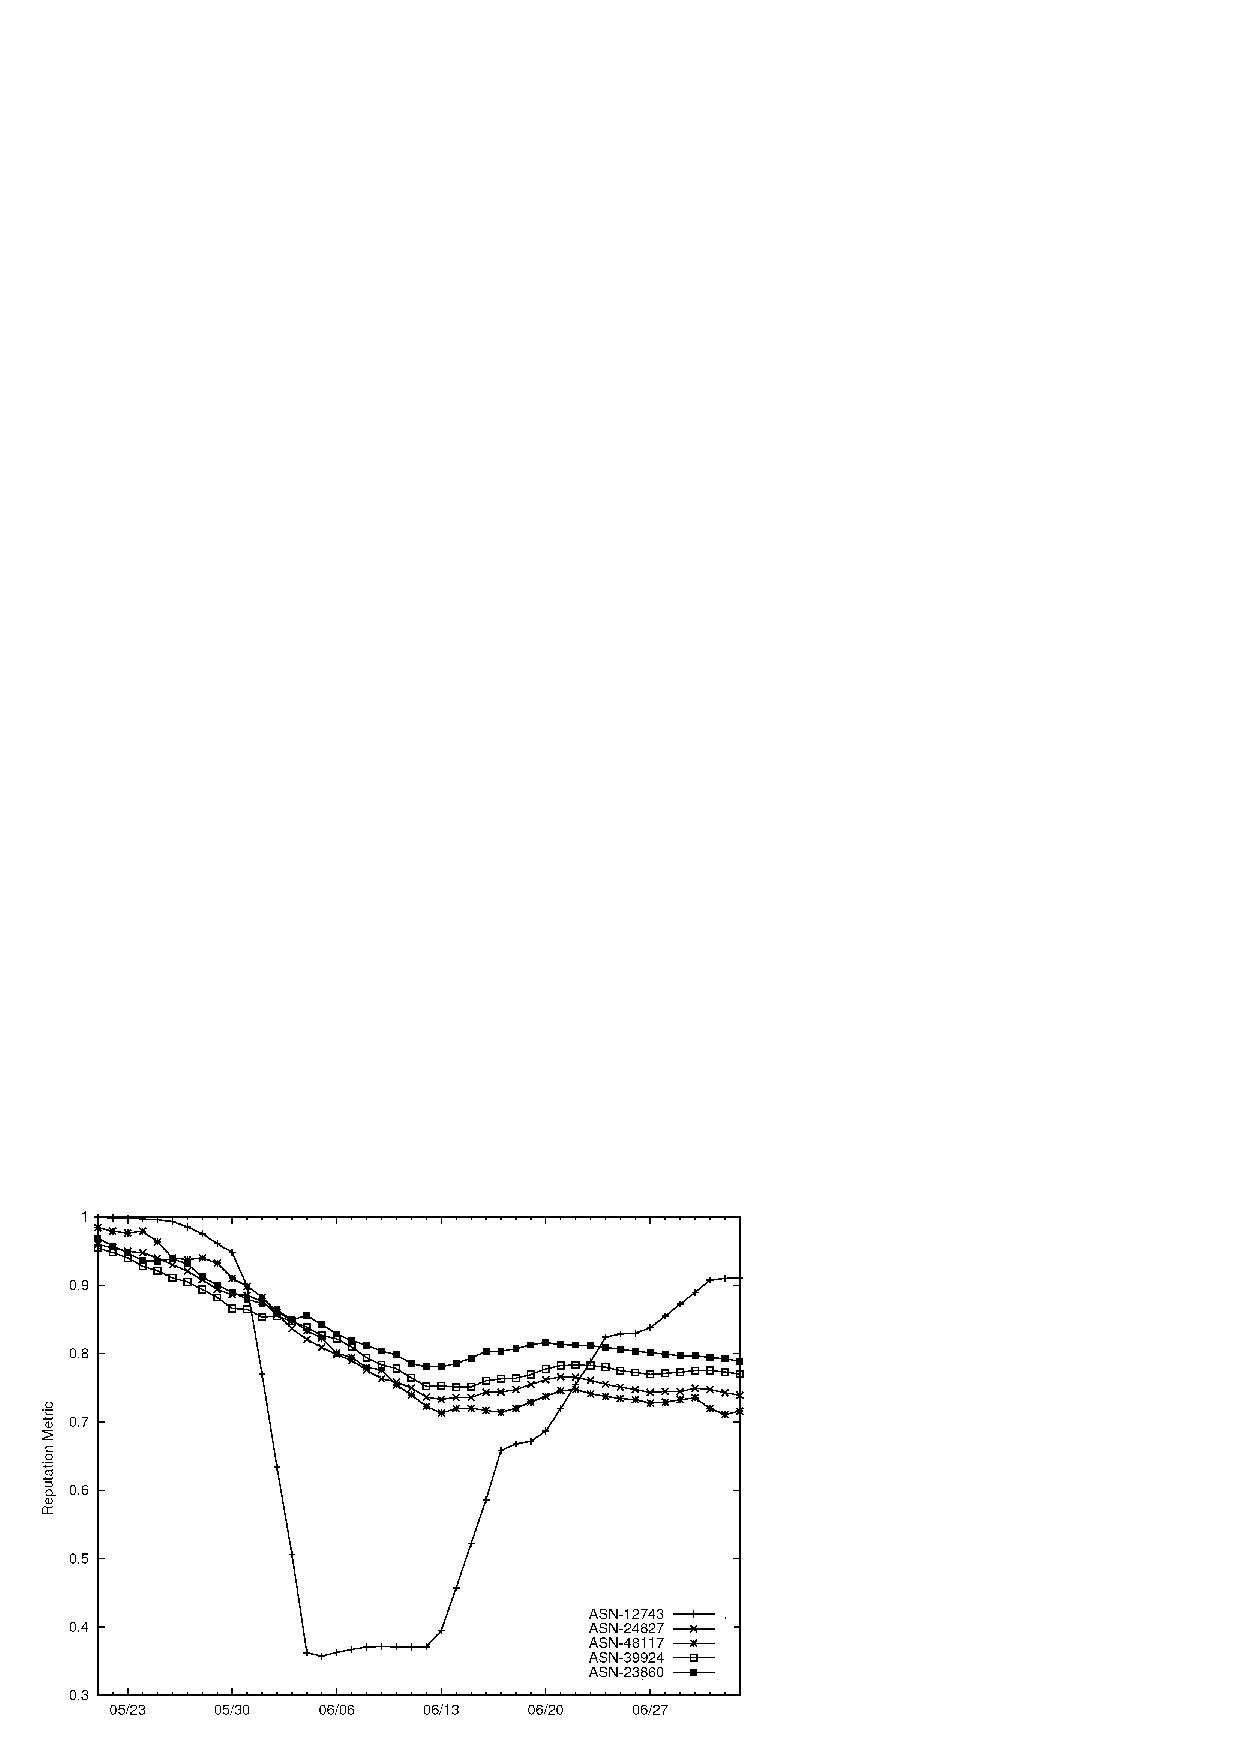
\includegraphics[width=0.75\linewidth]{some_graph}
	\end{center}
	\vspace{-12pt}
	\caption{Example Figure/Graph}
	\label{fig:some_graph}
\end{figure}

\end{document} 

